\documentclass[11pt]{report}
\usepackage{eso-pic,graphicx}
\usepackage[export]{adjustbox}
\usepackage{url}
\usepackage{amsmath}
\usepackage[top=2cm, bottom=2cm, outer=2cm, inner=2cm]{geometry}
\begin{document}
\AddToShipoutPictureBG*{
\includegraphics[width=\paperwidth,height=\paperheight]{images/bkgrnd}}
\begin{center}
\vspace*{2cm}
\textsf{\begin{Huge}
\textbf{ELP­718 ­ Telecom Software Laboratory \\
1st Semester, 2016-18 \\
Abhishek Mishra\\
27 Sep 2016, 5pm\\
Assignment-9}\\
\end{Huge}}
\vspace*{6cm}

\includegraphics[scale=0.12, center]{images/iitlogo}
\end{center}
\pagebreak
\tableofcontents
\vspace{5cm}
\pagebreak
\section{Introduction}
\vspace*{1cm}
This assignment aims to provide a better understanding of the following topics:\\
\begin{flushleft}
1. \textbf{Python}\\
Python is a widely used high-level, general-purpose, interpreted, dynamic programming language.[24][25] Its design philosophy emphasizes code readability, and its syntax allows programmers to express concepts in fewer lines of code than possible in languages such as C++ or Java.[26][27] The language provides constructs intended to enable writing clear programs on both a small and large scale.[28]

Python supports multiple programming paradigms, including object-oriented, imperative and functional programming or procedural styles. It features a dynamic type system and automatic memory management and has a large and comprehensive standard library.[29]

Python interpreters are available for many operating systems, allowing Python code to run on a wide variety of systems. Using third-party tools, such as Py2exe or Pyinstaller,[30] Python code can be packaged into stand-alone executable programs for some of the most popular operating systems, so Python-based software can be distributed to, and used on, those environments with no need to install a Python interpreter.

CPython, the reference implementation of Python, is free and open-source software and has a community-based development model, as do nearly all of its variant implementations. CPython is managed by the non-profit Python Software Foundation.
\end{flushleft}

\begin{flushleft}
2. \textbf{SQL}\\
MySQL is an open-source relational database management system (RDBMS). Its name is a combination of "My", the name of co-founder Michael Widenius' daughter,and , the abbreviation for Structured Query Language. The MySQL development project has made its source code available under the terms of the GNU General Public License, as well as under a variety of proprietary agreements. MySQL was owned and sponsored by a single for-profit firm, the Swedish company MySQL AB, now owned by Oracle Corporation. For proprietary use, several paid editions are available, and offer additional functionality.

MySQL is a central component of the LAMP open-source web application software stack (and other "AMP" stacks). LAMP is an acronym for "Linux, Apache, MySQL, Perl/PHP/Python". Applications that use the MySQL database include: TYPO3, MODx, Joomla, WordPress, phpBB, MyBB, and Drupal. MySQL is also used in many high-profile, large-scale websites, including Google (though not for searches), Facebook, Twitter, Flickr, and YouTube.

\end{flushleft}
\newpage
\section{Problem Statement}
Design a Database system for Bharti School which holds the details of the Student, Courses being float and the Students enrolled in those Courses.\\
The Relational tables required for this task are:\\
\begin{gather*}
\textbf{Student}(Stu\_id, Name, Gender);\\
\textbf{Course}(Course\_id, Course name, Instructor);\\
\textbf{Enroll}(Stu\_id, Course\_id);\\
\textbf{Grades}(Stu\_id, Course\_id, Grade);\\
\end{gather*}
	
\subsection{Assumptions}
The number of Courses being float are 8 only which are Signal Theory, Telecom Software Lab, Computer Networks, Telecom Technologies, Telecom Management System, Braodband Communication, Coding Theory, Digital Communication. \\
The Instructors are Prof. Subrat Kar, Prof. Ranjan Bose, Prof. Mahim Sagar, Prof. Shankar Prakriya.\\
A Student is allowed to enroll in atmost 4 Courses.\\
There is atleast a student in a Course.
\subsection{Part 1}
Design Database for given system using MySQL i.e. create one database and the relational tables described above. Also write a python code to populate the tables.\\
The generated table looks like this:\\
\begin{figure}[h!]
\centering
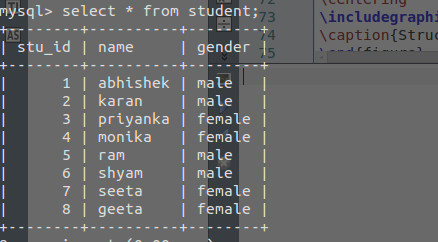
\includegraphics[scale=0.7]{images/part1stud}
\caption{Table Student}	
\end{figure}
\pagebreak
\begin{figure}[h!]
\centering
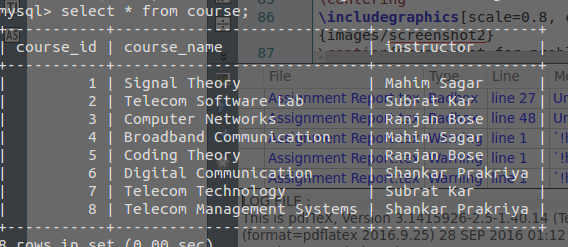
\includegraphics[scale=0.7]{images/part1course}
\caption{Table Course}	
\end{figure}
\pagebreak
\begin{figure}[h!]
\centering
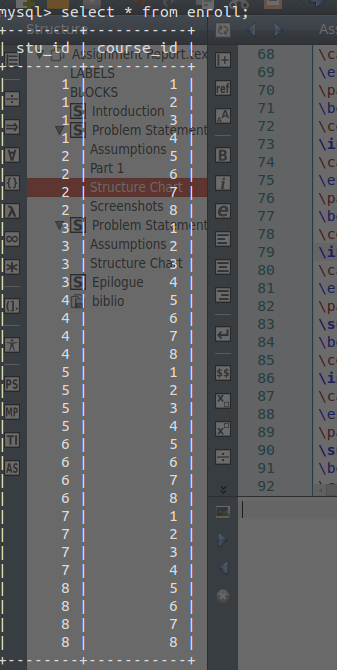
\includegraphics[scale=0.7]{images/part1enroll}
\caption{Table Enroll}	
\end{figure}
\pagebreak
\begin{figure}[h!]
\centering
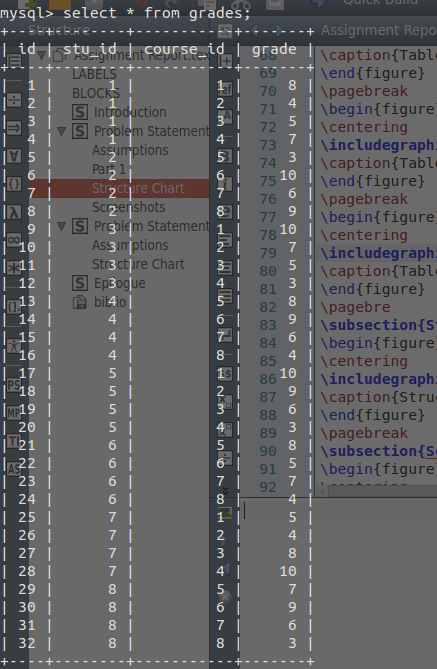
\includegraphics[scale=0.7]{images/part1grades}
\caption{Table Grades}	
\end{figure}
\pagebreak
\subsection{Part 2}
Write SQL query to find the names of those students who have enroll in both Coding theory and Telecom Management system.
\subsection{Part 3}
Write SQL query to find the names of those Students who have Scored an “A” in atleast one of the Subject taught by Prof. Subrat Kar.
\subsection{Part 4}
Write SQL query to find average grade for each of the course.
\subsection{Part 5}
Write SQL query to find the names of girl student who have topped in the course along with the course name.
\pagebreak
\subsection{Structure Chart}
\begin{figure}[h!]
\centering
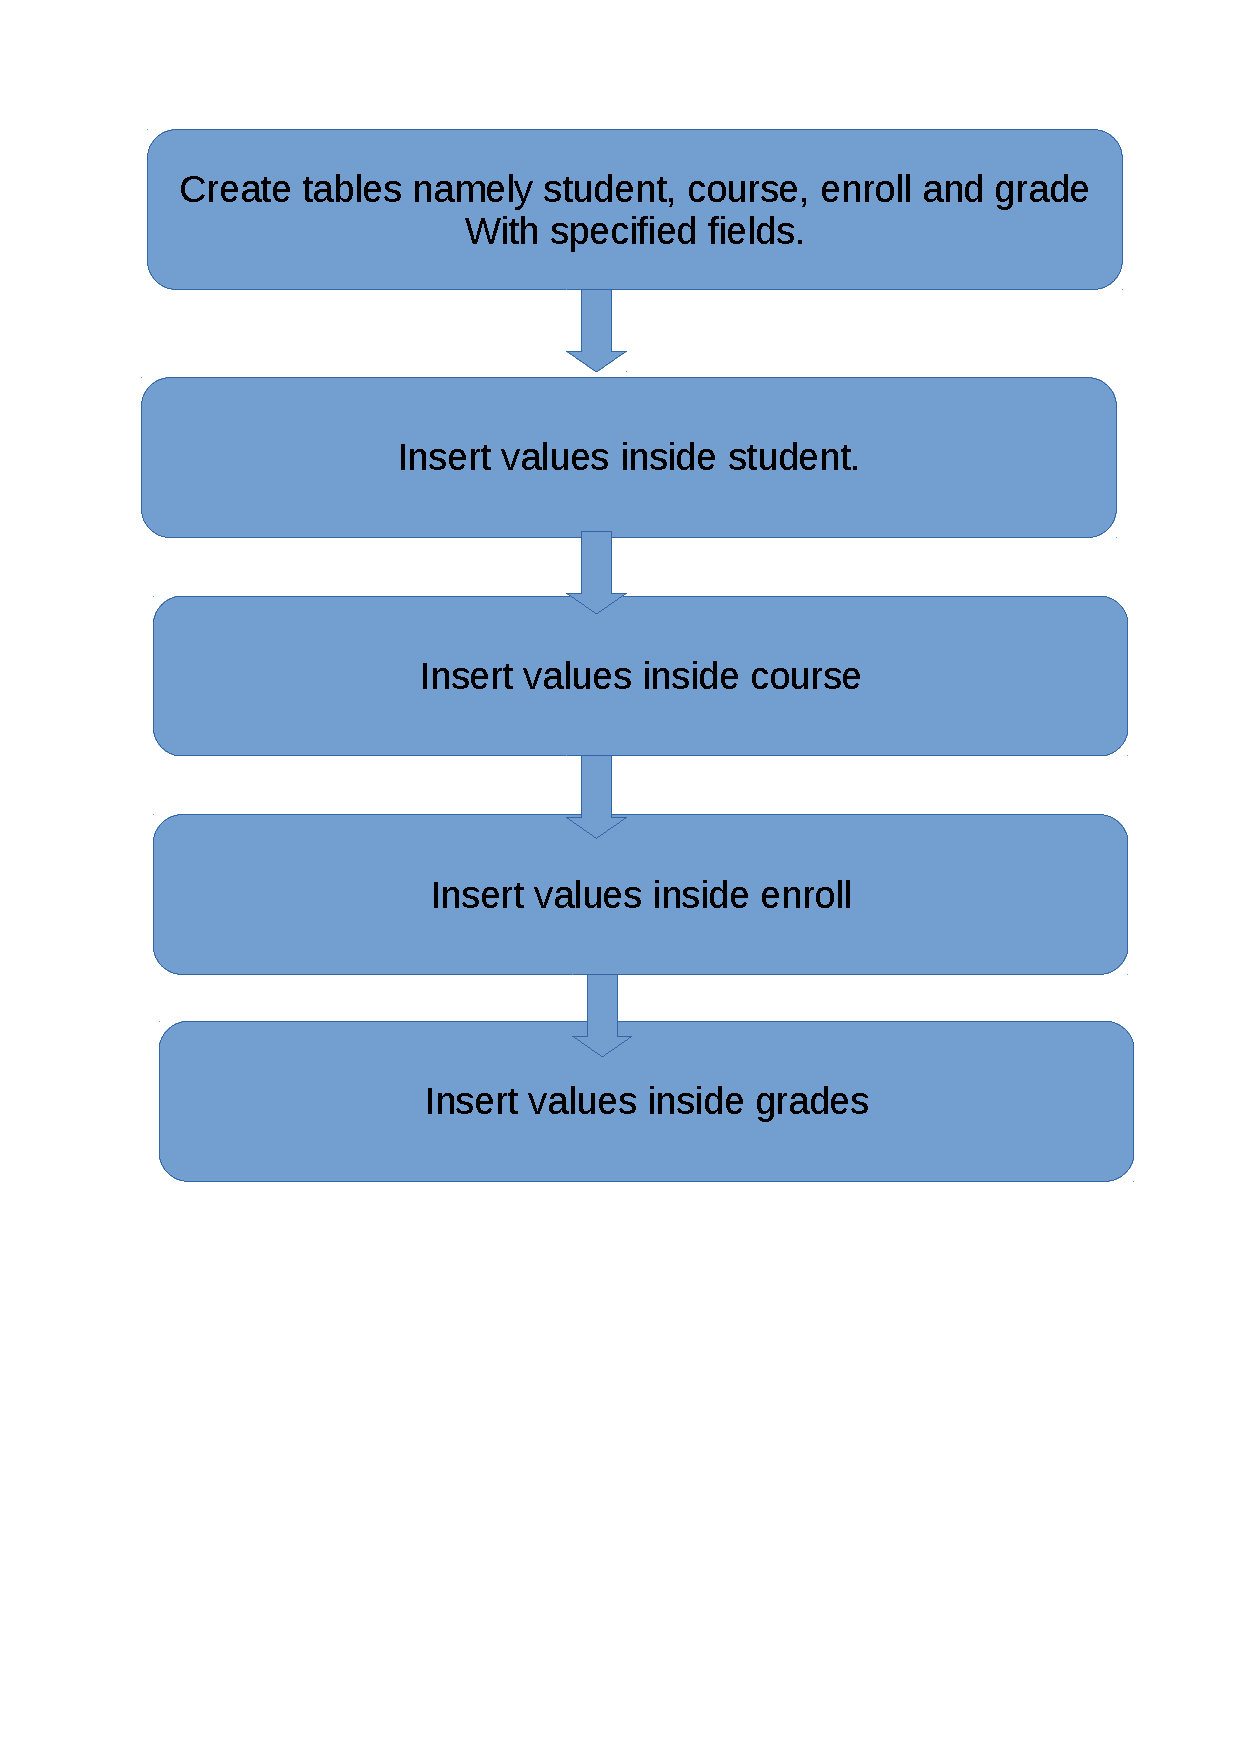
\includegraphics[scale=0.7]{images/sc1}
\caption{Structure chart for Part 1}	
\end{figure}
\pagebreak
\begin{figure}[h!]
\centering
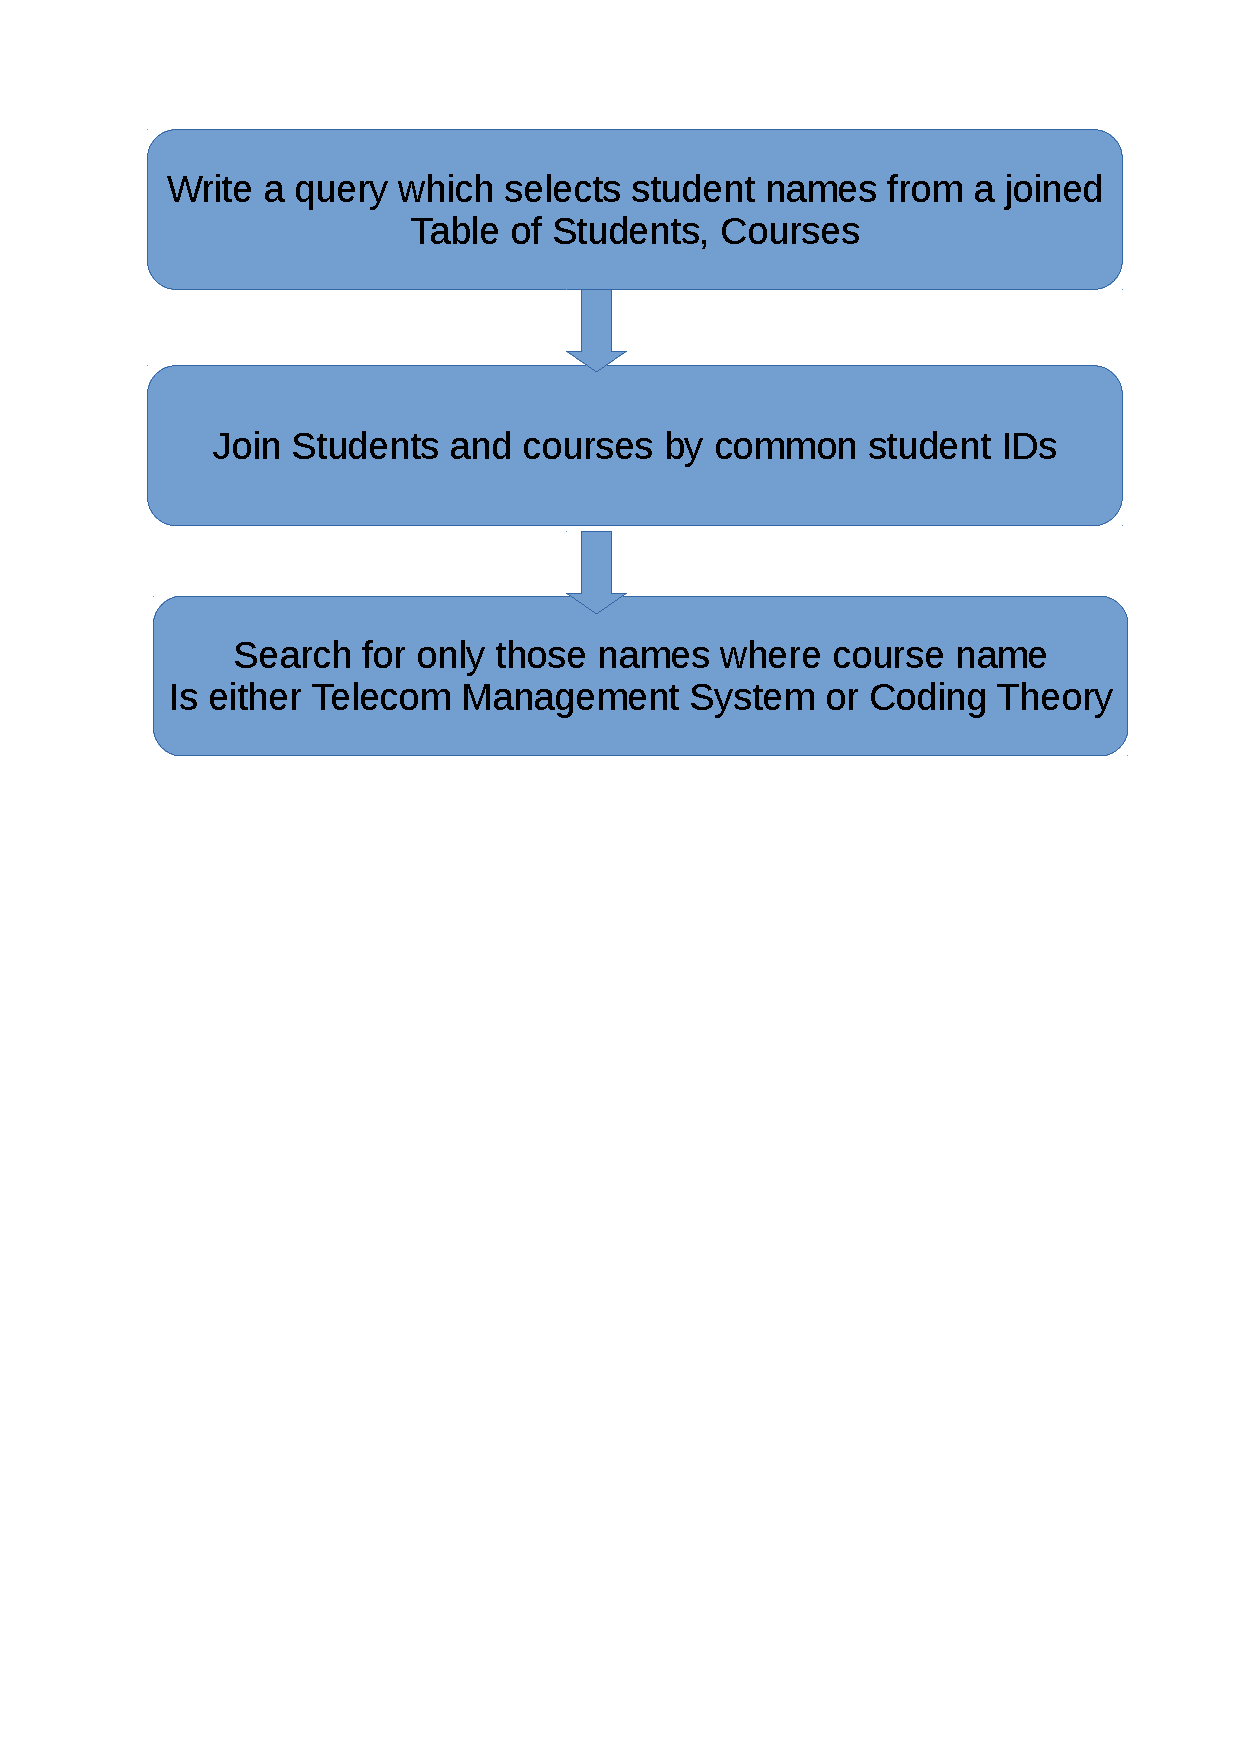
\includegraphics[scale=0.7]{images/sc2}
\caption{Structure chart for Part 2}	
\end{figure}
\pagebreak
\begin{figure}[h!]
\centering
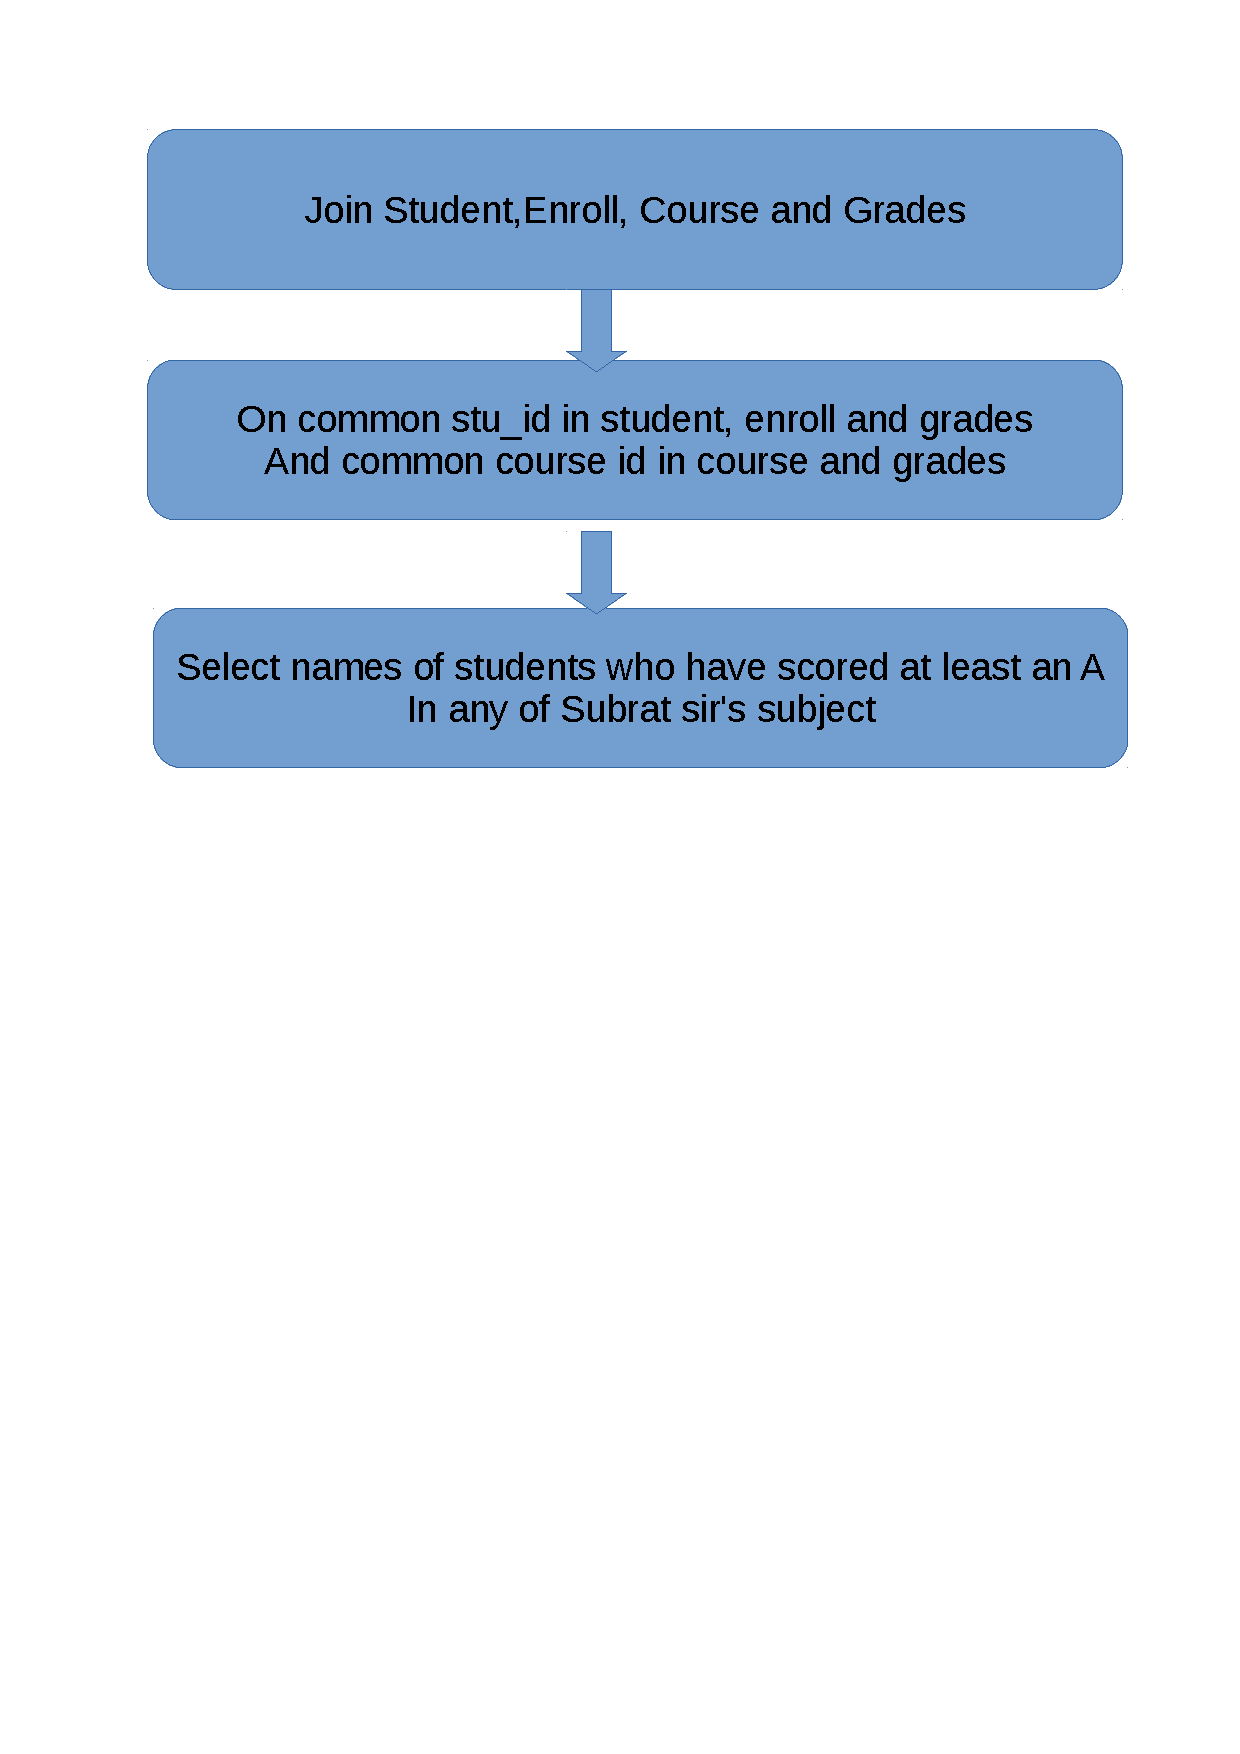
\includegraphics[scale=0.7]{images/sc3}
\caption{Structure chart for Part 3}	
\end{figure}
\pagebreak
\begin{figure}[h!]
\centering
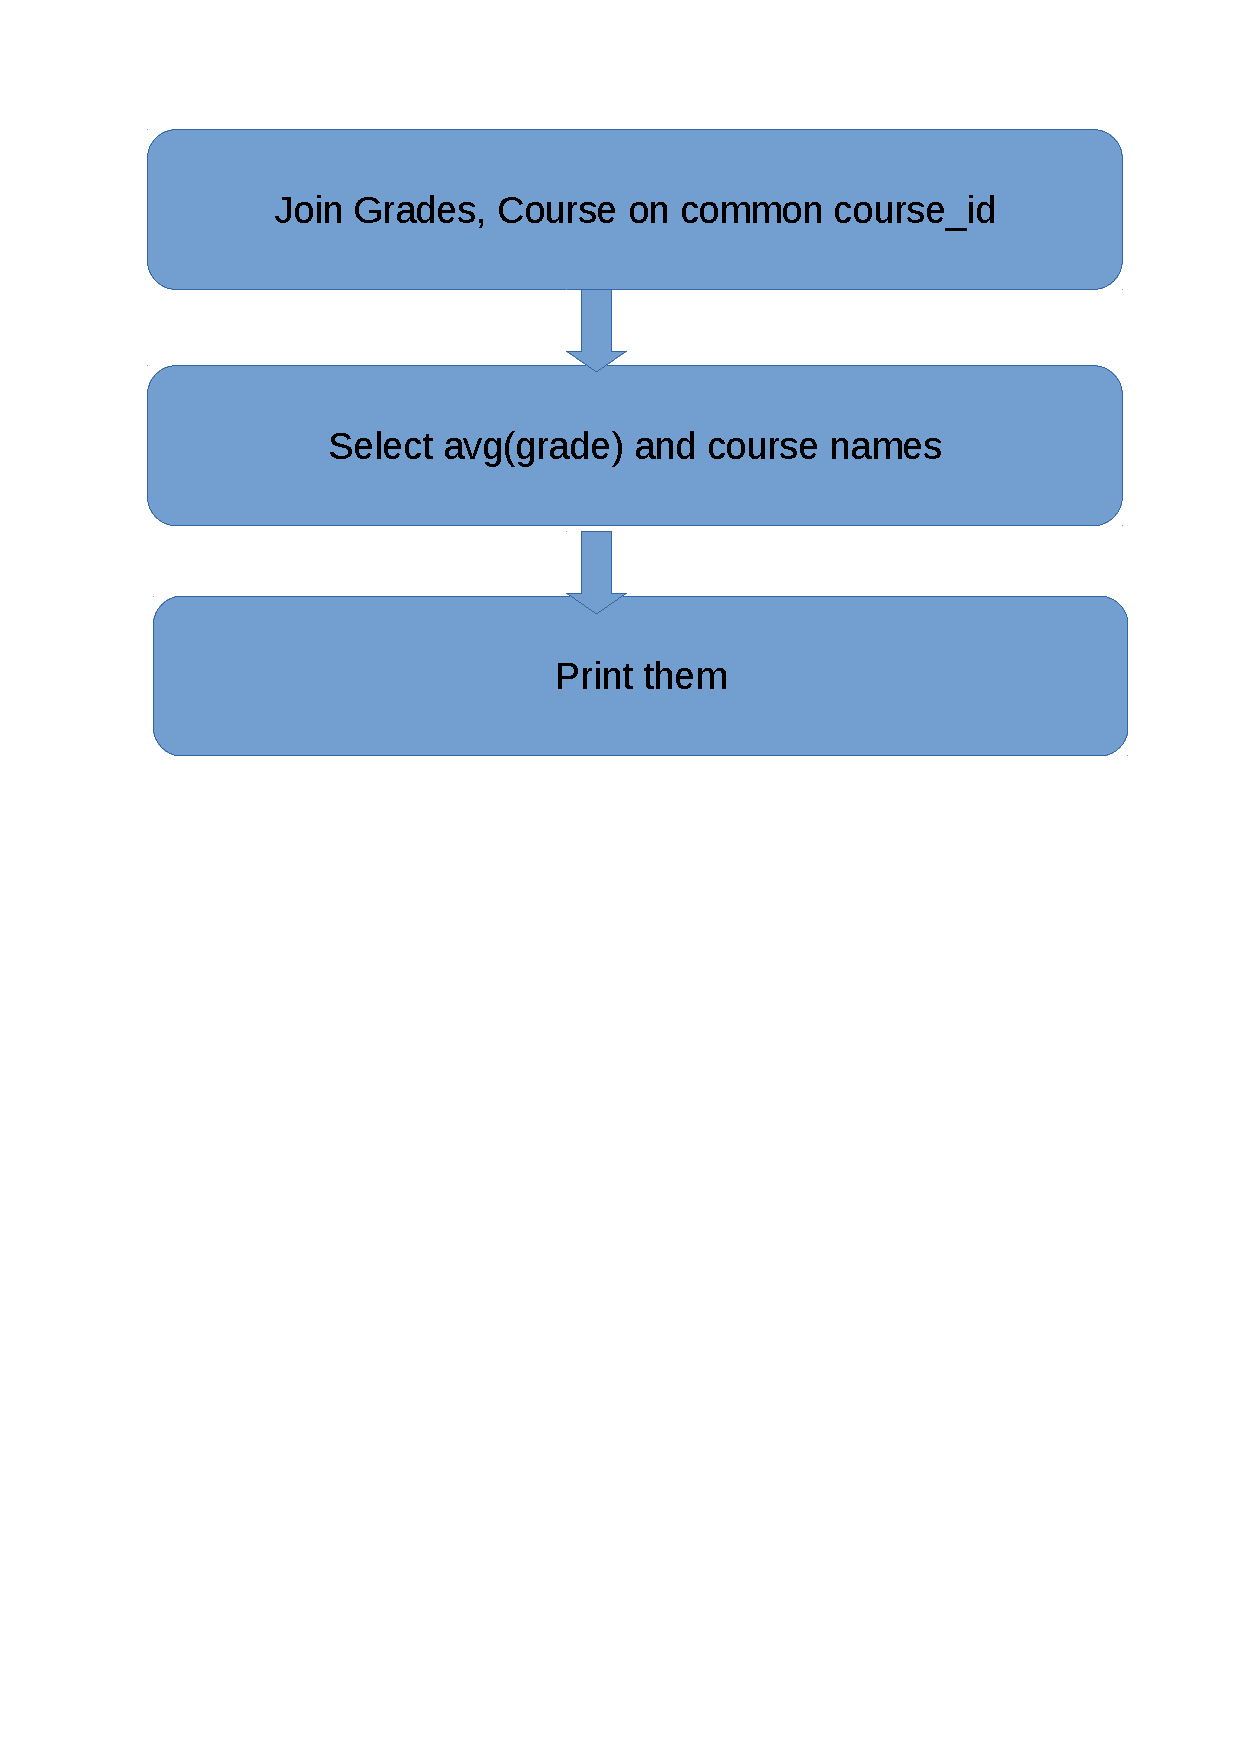
\includegraphics[scale=0.7]{images/sc4}
\caption{Structure chart for Part 4}	
\end{figure}
\pagebreak
\begin{figure}[h!]
\centering
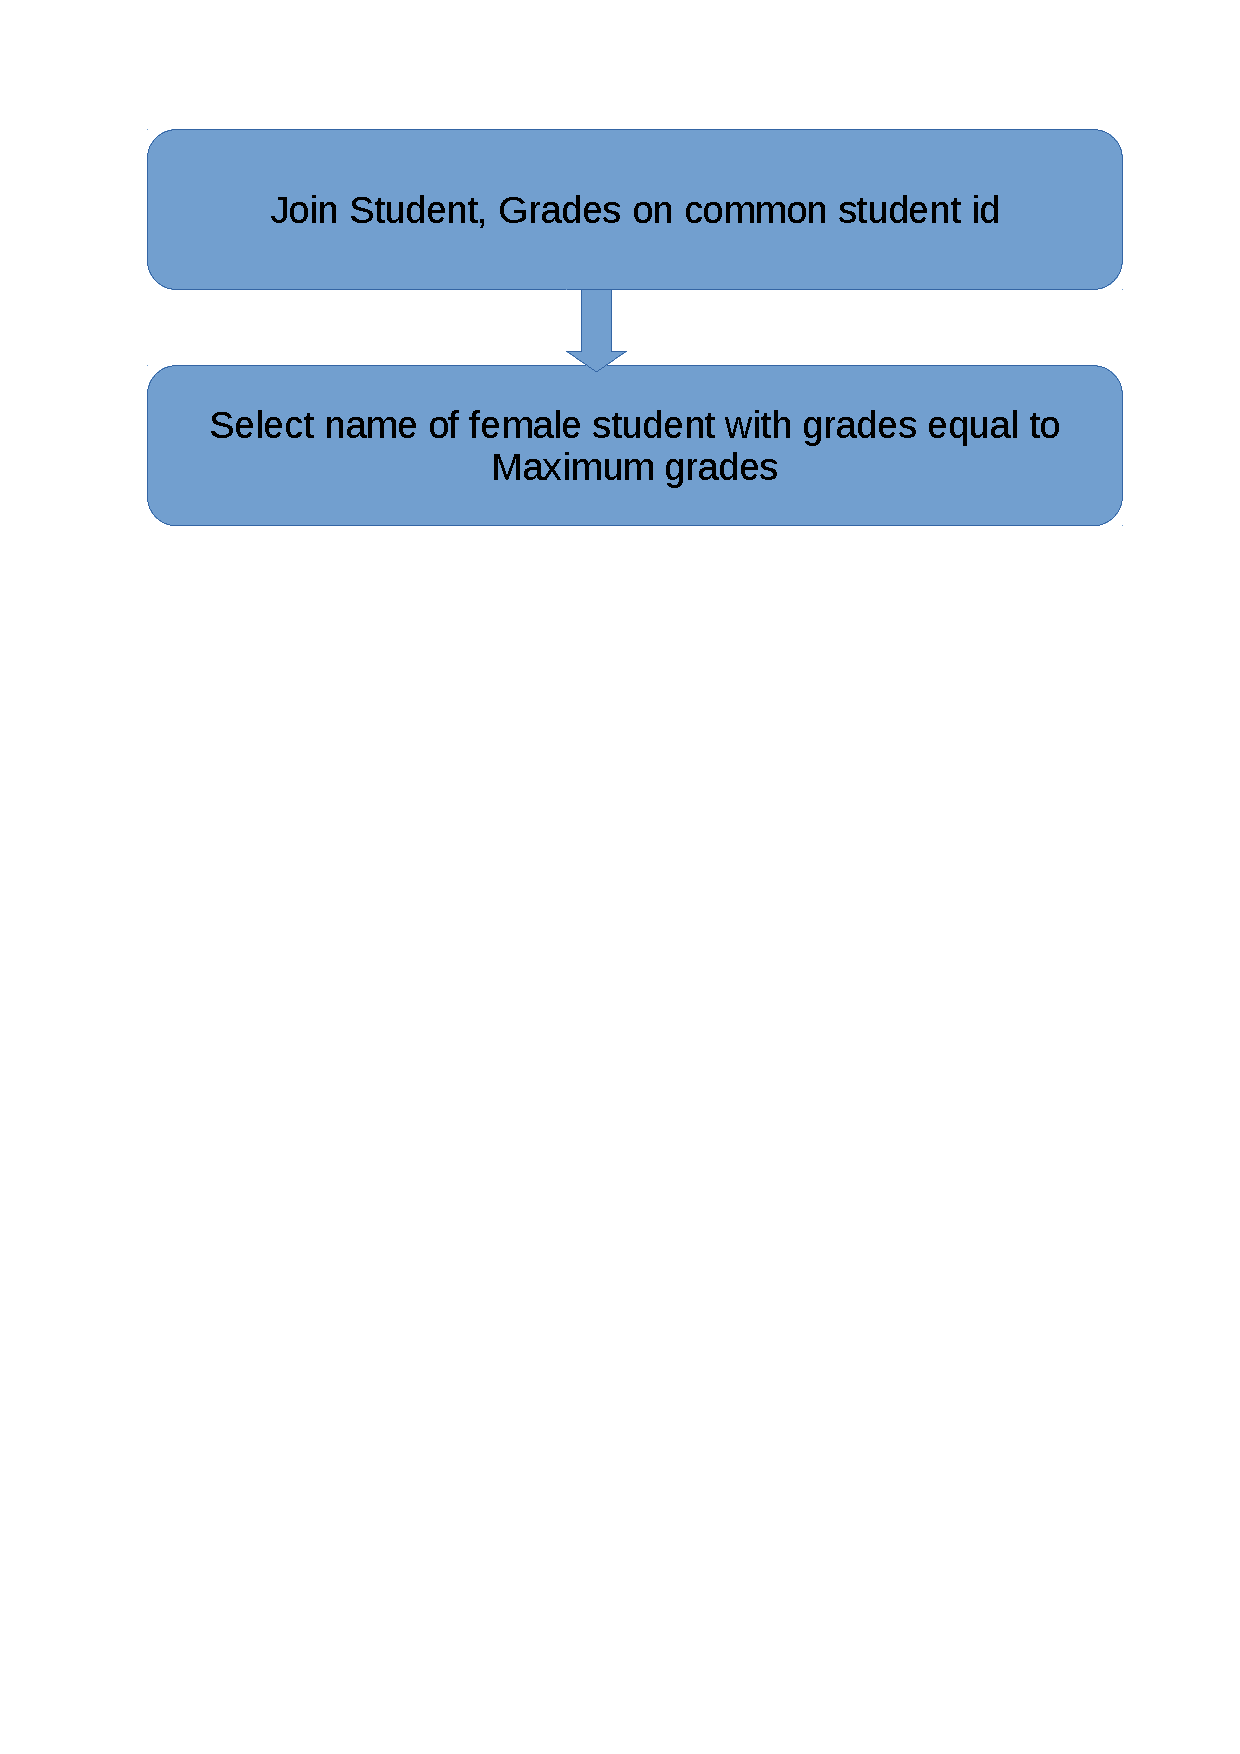
\includegraphics[scale=0.7]{images/sc5}
\caption{Structure chart for Part 5}	
\end{figure}
\pagebreak
\subsection{Screenshots}
\begin{figure}[h!]
\centering
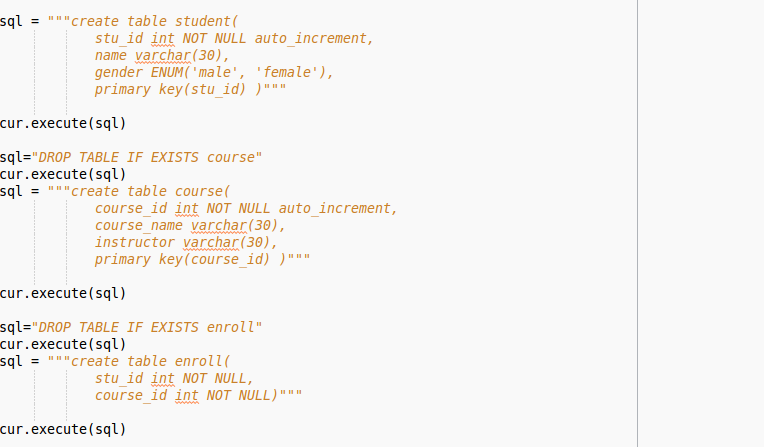
\includegraphics[scale=0.8, center]{images/screenshot1}
\caption{Screenshot for part 1}
\end{figure}
\pagebreak
\begin{figure}[h!]
\centering
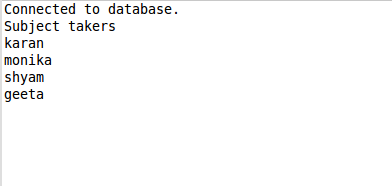
\includegraphics[scale=0.8, center]{images/screenshot2}
\caption{Screenshot for part 2}
\end{figure}
\pagebreak
\begin{figure}[h!]
\centering
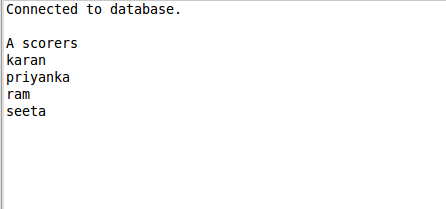
\includegraphics[scale=0.8, center]{images/screenshot3}
\caption{Screenshot for part 3}
\end{figure}
\pagebreak
\begin{figure}[h!]
\centering
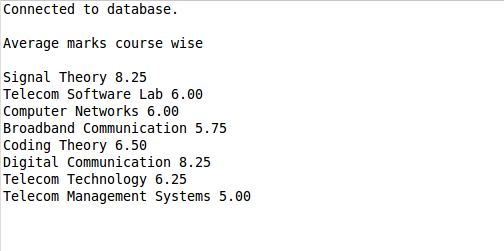
\includegraphics[scale=0.8, center]{images/screenshot4}
\caption{Screenshot for part 4}
\end{figure}
\pagebreak
\begin{figure}[h!]
\centering
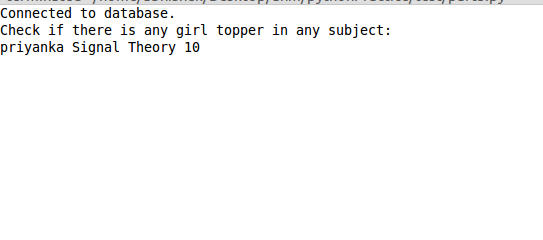
\includegraphics[scale=0.8, center]{images/screenshot5}
\caption{Screenshot for part 5}
\end{figure}
\pagebreak
\section{Epilogue}
This week's assignment tested our database management skills and our ability to form basic RDBMS relations and using them to execute our required tasks. 
\bibliography{biblio} 
\bibliographystyle{ieeetr}
\nocite{*}
\end{document}